%
% problemstellung.tex -- Beispiel-File für die Beschreibung des Problems
%
% (c) 2020 Prof Dr Andreas Müller, Hochschule Rapperswil
%
\section{Problemstellung
\label{quadratur:section:problemstellung}}
\rhead{Problemstellung}
\subsection{Überlegung hinter der Gauss-Quadratur \label{quadratur:subsection:ueberlegung}}

Bei der Integration mit der Trapez-/Mittelpunktregel kann man die Genauigkeit
der Annäherung verbessern, indem man mehr Teilintervalle berechnet.
Dabei werden mehr Stützstellen auf der $x$-Achse benötigt und mehr Funktionsauswertungen
müssen berechnet werden.

Die Wahl der Position und Anzahl Stützstellen stellt hierbei einer der beiden Freiheitsgrade
in der Berechnung des Integrals dar.
Der zweite Freiheitsgrad ist die Verwendung einer Gewichtung für eine spezifische Stützstelle.
Das Hinzuziehen einer Gewichtung erlaubt es, in einem Teilintervall, 
in dem die Annäherung stärkere Abweichungen zum eigentlichen Graphen hat, 
diese Abweichung zu minimieren. 


\subsubsection{Beispiel: Integration einer Funktion mit der Trapezregel}
Das folgende Beispiel illustriert die Integration für eine Funktion mit der Trapezregel und
zeigt die Verbesserung der Genauigkeit unter Verwendung von mehr Stützstellen oder einer Gewichtung.

\begin{figure}[!h]
    \centering
    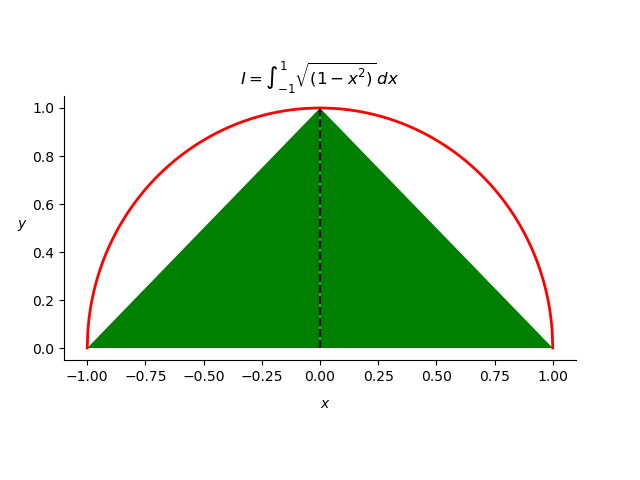
\includegraphics[scale=0.7]{papers/quadratur/figures/GaussTrapez1}
    \caption{Integration mit der Trapezregel mit drei Stützstellen
    \label{quadratur:figure:trapez1}} 
\end{figure}


In der Grafik~\ref{quadratur:figure:trapez1} sieht man die Integration der Funktion $I = \int_{-1}^{1}\sqrt{(1-x^2)}\,dx$
mit der Trapezregel mit drei Stützstellen an den Punkten $x=-1, x=0, x=1$.
Die Funktion $I$ beschreibt hierbei einen Halbkreis um das Zentrum $x=0$, 
dessen Fläche man geometrisch leicht ermitteln kann.
Die Fläche eines Halbkreises mit Radius $1$ ist $\frac{\pi}{2} \approx 1.570796$.
Betrachtet man nun die grün eingefärbte Fläche, sieht man zwei gleichschenklige rechtwinklige Dreiecke mit der Seitenlänge $1$,
somit lässt sich die grüne Fläche als ein Quadrat mit der Seitenlänge $1$ berechnen und erhält die Fläche $1$.

\newpage

\subsubsection{Beispiel: Gewichtung der Stützstellen}
Wird der Stützstelle $x=0$ das Gewicht $1.2$ gegeben, dann verhält sich die grüne Fläche wie zwei rechtwinklige Dreiecke 
mit den Seitenlängen $l_{x}=1, l_{y}=1.2$ und die resultierende Fläche lässt sich mit einem Rechteck mit den Seitenlängen
$a=1, b=1.2$ berechnen.
Man erhält die Fläche $1.2$ welche bereits etwas näher am tatsächlichen Resultat $\frac{\pi}{2} \approx 1.570796$ ist.

\subsubsection{Beispiel: Erhöhung der Anzahl Stützstellen}

\begin{figure}[!h]
    \centering
    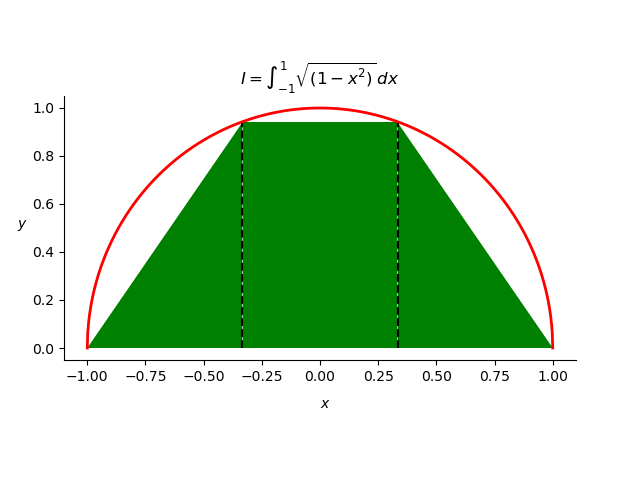
\includegraphics[scale=0.7]{papers/quadratur/figures/GaussTrapez2}
    \caption{Integration mit der Trapezregel mit vier Stützstellen
    \label{quadratur:figure:trapez2}}  
\end{figure}

\noindent
In der Grafik~\ref{quadratur:figure:trapez2} werden vier Stützstellen verwendet und man erhält zwei Teilintervalle mit 
rechtwinkligen Dreiecken mit den Seitenlängen $l_{x}=0.6666, l_{y}=0.94281$ und einem Rechteck mit den Seitenlängen
$l_{x}=0.6666, l_{y}=0.94281$. 
Die resultierende Fläche lässt sich mit der Formel $A= 2\cdot (l_{x} \cdot l_{y})$ berechnen 
und man erhält das Resultat $A=1.2571$.
Auch diese Annäherung weicht noch vom eingentlichen Resultat $\frac{\pi}{2} \approx 1.570796$ ab.

\noindent
Die Gauss-Quadratur basiert auf der Idee, dass die Stützstellen und deren Gewichtung so gewählt werden,
dass das Resultat optimiert wird und möglichst genau berechnet werden kann.
Dieses Verfahren erlaubt es, ein Polynom vom Grad $n$ mit nur $\frac{n-1}{2}$
Funktionsauswertungen exakt zu berechnen.

\newpage

\subsection{Anwendungsbereiche der numerischen Integration \label{quadratur:subsection:anwendungsbereiche}}
Die numerische Integration kann, wie im Kapitel~\ref{chapter:integration} beschrieben, dann verwendet
werden, wenn keine Stammfunktion in analytischer Form für eine Funktion gefunden werden kann.
Ein bekanntes Beispiel dafür ist die Verteilungsfunktion
\begin{equation}
    \phi(x) 
    =
    \frac{1}{\sqrt{2\pi}}
    \int_{-\infty}^x e^{-t^2/2}\,dt
\end{equation}
\noindent
der Standardnormalverteilung
\begin{equation}
    f(x)
    = 
    \frac{1}{\sigma \sqrt{2\pi}}e^{-\frac{1}{2}(\frac{x-\mu}{\sigma}^{2})}
\end{equation}
\noindent 
oder auch Gauss'sche Glockenkurve, wie in der Grafik~\ref{quadratur:figure:gaussdistribution} dargestellt. 

\begin{figure}[!h]
    \centering
    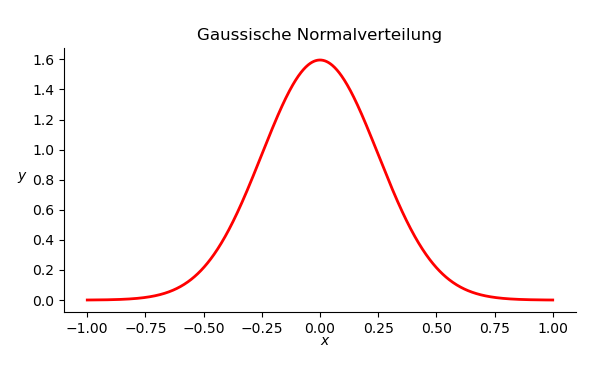
\includegraphics[scale=0.7]{papers/quadratur/figures/GaussDistribution1}
    \caption{Darstellung der Normalverteilung mit $\sigma=0.25$ und $\mu=0$
    \label{quadratur:figure:gaussdistribution}}
\end{figure}

\noindent
Weitere Beispiele mathematischer Funktionen ohne elementare Stammfunktionen können aus 
der Tabelle~\ref{buch:table:funktionenohnestammfunktion} entnommen werden.

\begin{table}[h!]
    \centering
    \begin{tabular}{|c|c|}
        \hline
        $\displaystyle \frac{\sin(x)}{x}$ & $\displaystyle \frac{x}{\sin(x)}$ \\
        \hline
        $\displaystyle \frac{e^{x}}{x}$ & $\displaystyle \frac{1}{\operatorname{ln}(x)}$ \\
        \hline
        $\displaystyle \frac{x}{\operatorname{ln}(x)}$ & $\displaystyle \operatorname{ln}(\sin(x))$ \\
        \hline
        $\displaystyle e^{x}\cdot\operatorname{ln}(x)$ &  \\
        \hline
    \end{tabular}
    
    \caption{Funktionen ohne elementare Stammfunktion
    \label{buch:table:funktionenohnestammfunktion}}  
    
\end{table}